\documentclass[../../../../document.tex]{subfiles}

\begin{document}
    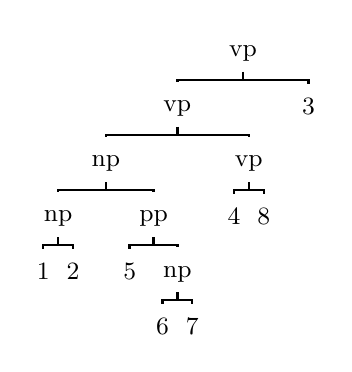
\begin{tikzpicture}[
        level distance=7mm,
        font=\small,
        sibling distance=10mm,
        anchor=center,
        every node/.style={text height=2.5mm},
        rounded corners=0,
        baseline=(mid.base)
        ]
        \begin{scope}[edge from parent path={(\tikzparentnode.south) -- ++(0,-1mm) -| (\tikzchildnode.north)}, every path/.style={line width=.2ex}]
            \node (croot) {\cn{vp}}
            [sibling distance=11ex]
            child { node {\cn{vp}}
                [sibling distance=12ex]
                child { node {\cn{np}}
                    [sibling distance=8ex]
                    child { node {\cn{np}}
                        [sibling distance=2.5ex]
                        child { node {1}}
                        child { node {2}}}
                    child { node {\cn{pp}}
                        [sibling distance=4ex]
                        child { node {5}}
                        child { node {\cn{np}}
                            [sibling distance=2.5ex]
                            child { node {6}}
                            child { node {7}}}}}
                child { node {\cn{vp\binsym{}}}
                    [sibling distance=2.5ex]
                    child {node {4}}
                    child {node (mid) {8}}}}
            child { node {3}};
        \end{scope}
    \end{tikzpicture}
\end{document}